\documentclass[prl, aps, 10pt, showkeys, twocolumn, nofootinbib]{revtex4-1}

\usepackage[cp1251]{inputenc}
\usepackage[english]{babel}
\usepackage{amsmath}
\usepackage{amssymb}
\usepackage{graphicx}

\bibliographystyle{apsrev4-1}

\DeclareMathOperator{\Li}{Li}
\DeclareMathOperator{\csch}{csch}

\begin{document}

\title{Electrons distribution on deformed liquid helium film}

\author{B.\,I.~Lev}
\author{V.\,P.~Ostroukh}
\author{V.\,B.~Tymchyshyn}
\author{A.\,G.~Zagorodny}
\affiliation{Bogolyubov Institute for Theoretical Physics}


\begin{abstract}
It is known that homogeneous distribution of charge for two-dimensional electron systems is unstable. Some structures, like bubblons and periodical modulations are formed.
This work proposes some simple quasi-classical model, that describes electrons behaviour and can predict some parameters of structures they form. 
Free energy functional for prototype system is obtained and, due to it, electron density distributions are got. 
Theory can be easily generalized for other systems of interacting particles.
\end{abstract}

\keywords{liquid helium, electrons, bubblon, two-dimensional electron systems}

\maketitle

\section*{Introduction}

Low-dimensional systems are now of the great interest to physicists.
This is caused by their simplicity, in contrast to three-dimensional systems, and lots of new physical effects, that reveal itself due to reduced dimensions.
Balls moving on the plane can be a classical example of the two-dimensional system, because their movement in third dimension ($z$-axis) can be neglected compared to the motion in $x$-$y$ plane.
Such systems are often called mesoscopic.


There are a lot of mesoscopic systems that can be experimentally studied.
They are known to be realized in emulsions, foams, polymers, colloidal suspensions, liquid crystals...
Much prominence is given by this article to some special case of mesoscopic system, namely electrons on the surface of dielectric substrate.


On the surface of dielectric substrate electrons have only two degrees of freedom \cite{edelman,ando_fowler_stern}.
Though, this number can be decreased even more.
The simplest way is to put surface of helium into perpendicular to it magnetic field.
This field causes Landau quantisation, so electrons begin moving by circular orbits, having effectively zero degrees of freedom.
Such systems are called quantum dots.
Ideally there must be only one electron in quantum dot, but now it is possible to study only quantum dots with several thousand of electrons \cite{alhassid}.


One-dimensional systems, called often quantum wires, are of a great interest because there is a possibility to detect Luttinger liquid \cite{luttinger} in such a kind of systems.
They can be created, for example, using nanotubes.
In liquid helium they can be observed by means of substrate with appropriate surface.
Electrons rearrange on the liquid helium surface to follow pattern substrate surface has.


Some features of using heterostructure, when studying two-dimensional electron systems were analysed theoretically in \cite{kroemer}.    
However, first experimental results in this field were received only few years later \cite{rupprecht_woodall_pettit}.
At the same time a possibility of creating a two-dimensional mesoscopic system on the surface of dielectric was predicted \cite{cole, cole_cohen, shikin}.
Year later first experiments have been carried out \cite{williams_crandall_willis}.
Since that time two-dimensional electron systems are extensively studied, and lots of interesting results are obtained.
Some of them were first predicted theoretically, like the Wigner crystallization, \cite{wigner,platzman_fukuyama,grimes_adams} and others\,--- first observed experimentally, like integer and fractional Hall effect \cite{klitzing_dorda_pepper, tsui_stormer_gossard, laughlin}.


Research of this system is in development now.
Different theories can predict different, sometimes mutually exclusive effects.
For example some theoretical researches show that in the absence of magnetic field electrons on a liquid helium surface should be an insulator \cite{abrahams_etc}, but other disagree with this point of view \cite{tanatar_hakioglu}, therefore, leaving some chances for superconductivity observation in this system.


Modern researches in this field are based mostly on quantum field theory \cite{zinn-justin} and scaling theory.
For example, electron transport properties in heterostructures can be researched using QFT methods as in \cite{datta} and more specifically for electrons on a liquid helium surface we can refer to \cite{monarkha_kono}.
As for the scaling theory, it was developed in \cite{thouless}.
The latter results are interesting as applicable to systems with different dimensions as far as the last one is an ordinary parameter in such a kind of models.
Nevertheless, these models are still complex and it can be interesting to build some simple quasiclassical model that covers some these system's properties.


This system is interesting not only because of being mesoscopic, but as a representative of a wide class of systems with Coulomb-like interaction.
These systems can significantly differ by physical properties, but their interparticle interaction is resembling Coulomb interaction.
One of many possible examples can be dusty plasma.
Electrons on the liquid helium surface and dust particles in plasma are much alike.
Dust particles even can form some stable periodical structures similar to Wigner crystall and undergo melting or crystallization \cite{GrainDynamics, StronglyCollisional}.
This process can even be accompanied with some kind of hysteresis \cite{myPublication}.


In this article we will try to look at electrons on the liquid helium surface in a way more typical for Coulomb-like systems.
On the other hand we will develop all the necessary formalism basing on modern research in the field of statistical equilibrium description of such a kind of systems in the terms of mean field extrapolation \cite{krasnoholovets_lev}.
These methods will be used to develop some simple quasiclassical model that describes electron behavior and can predict parameters of structures they form depending on external electric field intensity and temperature.
We will obtain electrons distribution function and conditions for distribution to be changed from the uniform one to periodic and bubbles to be formed.


These studies are not only of academic interest but can have some practical applications.
For example, it is proposed to use this system for quantum computations \cite{platzman_dykman}.


Next sections are ordered as follows.
First we develop some general formalism for the statistical equilibrium description for such systems in the mean-field extrapolation.
Then we introduce model we will be using and, of coarse, assumption we can do to simplify it's consideration.
Subsections in this section are providing application of the general formalism to the model under consideration taking possible assumptions and simplifications into account.
Therefore the result is still to general (we are not using the explicit form of the interparticle potential till this point) the last subsections are providing electron-electron potential and possible form of electron density function consideration.
It should be mentioned, that we are adding there some additional effective potential, that is a result of the helium film deformation.
Results of the computer simulation considered next show, that this summand can cause significant change of the electrons distribution function and should be taken into account.
Last sections are devoted to possible additional simplifications that can make this model analytically considerable and to computer simulation results. 



\section{Satistical mechanics for systems of particles with interaction}

%TODO add intro

%In this section we will develop a general formalism for quantum systems with interaction 


It is known from statistical physics that stable states of systems minimize its free energy. 
So, first of all we should find an expression for it.
Though, we wouldn't specify our system until we don't need it. 
So, we will get rather general theory, that can be extended to a lot of systems.


For a wide number of systems hamiltonian can be written in form:
$$ 
  H(n) = \sum_s \epsilon_s n_s + \frac12 \sum_{s,s^{\prime}} V_{ss^{\prime}} n_s n_{s^{\prime}}.
$$
Here $\epsilon_s$ --- additive part of particle energies (Usually it is kinetic energy, but also it can be an energy in external field.), $s$ indicates particle states, $V_{ss^{\prime}}$ is interaction energy between particles in states $s$ and $s^{\prime}$, $n_s$ --- ocupation number of state $s$. 
Now we can write partition function of such system:
$$
  \begin{aligned}
    Z % =
      &= \sum_{\{n_s\}} \exp (-\beta H) % =
	= \sum_{\{n_s\}} \exp \Biggl[ 
	  - \beta \Biggl(
	      \sum_s \epsilon_s n_s + 
	  \Biggr.
	\Biggr. \\
      &+ \Biggl.
	 \Biggl.
              \frac{1}{2} \sum_{s,s^{\prime}} V_{s s^\prime} n_s n_{s^\prime}
        \Biggr) 
    \Biggr].
\end{aligned}
$$
To perform formal summation in this equation, we shall use well-known properties of gaussian integrals over auxiliary fields:
$$
\begin{aligned}
\exp \left( 
         \frac{\nu^2}{2 \vartheta} \sum_{s,s'} \omega_{ss'} n_s n_{s'} 
     \right) &= 
\int\limits_{-\infty}^{\infty} D\varphi \exp \Biggl( 
    \nu \sum_s n_s \varphi_s - \Biggr. \\
   &- \Biggl.
        \frac{\vartheta}{2} \sum_{s,s'} \omega_{ss'}^{-1} \varphi_s \varphi_{s'} 
    \Biggr),
\end{aligned}
$$
with 
$D \varphi = \frac{\prod_s d\varphi_s}{\sqrt{\det(2 \pi \beta \omega_{ss'})}}.$ 
Now we escape quadratic dependence on occupation numbers of states, carrying it to introduced field\footnote{In the future infinite limits of integration will be omited.}:
$$
Z = \int D\varphi \exp \left[
        \sum_s (i \varphi_s - \beta \epsilon_s) n_s -
           \frac{1}{2\beta} \sum_{s,s'} \left( 
           V_{ss'}^{-1} \varphi_s \varphi_{s'} 
       \right) 
    \right].
$$
We shall assume canonical ensemble now. 
To fix number of particles in system we'll use Cauchu formula: 
$$
\frac{1}{2 \pi i} \oint \xi^{\sum_s n_s - N - 1} d\xi = 1.
$$
After this we get partition function for N-particle system:
$$
\begin{aligned}
Z_N &= \frac{1}{2 \pi i} 
       \oint d\xi \int D\varphi \exp\Biggl[ 
          - \frac1{2\beta} \sum_{s,s'}
                V_{ss'}^{-1} \varphi_s \varphi_{s'} - 
       \Biggr.\\
    &  \Biggl. 
          - (N+1) \ln\xi 
       \Biggr] \prod_s \sum_{\{n_s\}} \left[
           \xi \exp(i \varphi_s - \beta \epsilon_s)
       \right]^{n_s}.
\end{aligned}
$$
We can perform summation in obtained equation, according to the type of statistics. 
We get:
$$
Z_N = \frac1{2 \pi i} \oint d\xi \int D\varphi \exp [
        - \beta F(\varphi,\xi)],
$$
with free energy:
\begin{equation}
\label{betaF0}
\begin{aligned}
  \beta F&(\varphi,\xi) 
= \frac1{2\beta} \sum_{s,s'} V_{ss'}^{-1} \varphi_s \varphi_{s'} + \\
&+ \delta \sum_s \ln \left(
       1 - \delta \xi e^{-\beta \epsilon_s+i \varphi_s}
   \right) + (N+1) \ln \xi . 
\end{aligned}
\end{equation}
Variable $\delta$ indicates type of statistics that we have. It equals $+1$ for Bose-Einstein statistics, $0$ for Maxwell-Boltzmann statistics and $-1$ for Fermi-Dirac statistics.


We have got an expression for free energy of system of interacting partilles in presentation of gauge fields. It also depends on chemical activity of particles $\xi = \exp ( \beta \mu )$. Now we should perform summation in it. Due to complexity of expression we can't do it directly, so we should make some approaches. Let's make concideration that main contribution to the partition function is made by states that correspond to the saddle point.
Saddle-point conditions for our system can be written as:
$$
  \frac{\delta \beta F}{\delta \varphi}
= \frac{\delta \beta F}{\delta \xi} 
= 0.
$$
After the variation of (\ref{betaF0}) we have got system for determination of saddle-point states:
\begin{subequations}
\begin{eqnarray}
  &\frac1{\beta} \sum_{s'} V_{ss'}^{-1} \varphi_{s'} 
- \frac{i \xi e^{-\beta\epsilon_s + i \varphi_s}}
       {1 - \delta\xi e^{-\beta\epsilon_s + i \varphi_s}} 
= 0; \label{saddle1}\\
  &\sum_s \frac{\xi e^{-\beta \epsilon_s + i \varphi_s}}
              {1 - \delta \xi e^{-\beta \epsilon_s + i \varphi_s}} 
= N+1.  \label{saddle3}
\end{eqnarray}
\end{subequations}
As we can see from (\ref{saddle3}), expression
\begin{equation}
  \label{f_s}
  f_s = \frac{\xi e^{-\beta\epsilon_s + i \varphi_s }}
           {1 - \delta\xi e^{-\beta\epsilon_s + i \varphi_s}}
\end{equation}
can be treated as averaged occupation numbers of the states. 


Obtained system gives us possibility to get dirrectly saddle-point states, that can be interpreted as thermodynamically stable distributions.
Thus, in such method of their calculation mathematical difficultnesses appear.
As we can see, there is inverce ineraction matrix in equation (\ref{saddle1}).
Its determination is difficult mathematical problem itself.
It is known \cite{edwards_lennard, samuel} for potentials of the form $\omega_{ss^{\prime}} = \omega(|\vec{r}_s - \vec{r}^{\prime}_s|)$ in continuous case that inverce interaction matrix is given by:
$$
\omega_{ss^{\prime}}^{-1} = \delta_{ss^{\prime}} \hat{L}_{r^{\prime}},
$$
where $\hat{L}_{r'}$ is operator, for which the interaction potential is Green function.
We know inverce operator for the screened Coulomb potential \cite{edwards_lennard, hubbard, samuel}:
\begin{equation}
\hat{L}_{r'} = -\frac{1}{4 \pi q^2} (\Delta_{r'} - \lambda^2),
\end{equation}
where $q^2$ is interaction constant and $\lambda^{-1}$ is the screening length.
Problem of some particular potentials have been solved in~\cite{lev_zhugayevich}.


For more general interaction potential inverce operator is unknown, so we should find a way to turn back to the dirrect operators.
This possibility is given us by (\ref{f_s}). Using this expression, we can do inverce transformation to the occupation numbers:
$$
\begin{aligned}
&\varphi_s = i \beta \sum_{s'} V_{ss'} f_{s'},\\
&\frac1{2\beta} \sum_{s,s'} V_{ss'}^{-1} \varphi_s \varphi_{s'} 
  = - \frac{\beta}2 \sum_{s,s'} V_{ss'} f_s f_{s'},
\end{aligned}
$$
and rewrite free energy:
\begin{equation}
\label{betaF1}
\begin{aligned}
 \beta F[f,\xi] 
= - \frac{\beta}{2} \sum_{s,s'} V_{ss'} f_s f_{s'} 
 &- \delta \sum_{s} \ln (1 + \delta f_s) \\
 &+ (N+1) \ln \xi (f).
\end{aligned}
\end{equation}
For canonical ensemble we should escape chemical potential in this formula. We can get it from (\ref{f_s}):
$$
\ln\xi(f) \equiv \beta\mu = \beta(\epsilon_s + E_s) + \ln f_s - \ln (1 + \delta f_s).
$$
with
\begin{equation}
\label{mean_field}
E_s = \sum_s V_{ss'} f_{s'}.
\end{equation}
We concider chemical potential to be constant throughout the system, but it is convenient to take it as simple average through all states:
$$
\ln \xi (f)
     = \frac{1}{N}\sum_s f_s \left[ 
           \beta(\epsilon_s + E_s) + \ln f_s - \ln (1 + \delta f_s) 
       \right].
$$
Now we can put this into the free energy (\ref{betaF1}) and get:
\begin{equation}
\label{free_energy}
\begin{aligned}
   \beta F[f] 
&= \beta \sum_s f_s \epsilon_s 
 + \frac{\beta}{2} \sum_{s,s'} V_{ss'} f_s f_{s'} + \\
&+ \sum_s \left[f_s \ln f_s - (f_s+\delta) \ln (1 + \delta f_s) \right].
\end{aligned}
\end{equation}
This expression can be easily interpreted. First item is kinetic energy of a system, second -- potential energy of interacting particles. Third is contribution of entropy, and it equals zero for $T=0.$


Now we can check correspondense of our theory to the classical results. Let us now concider grand canonical ensemble. For fixed chemical potential we can get from (\ref{f_s}) generalisation of well-known distributions:
$$
f_s = \frac{1}{e^{\beta (\epsilon_s + E_s - \mu) } - \delta}, \label{rozp_uzag0}
$$
Together with (\ref{mean_field}) it can be used for numerical finding of stable states with iteration method. This expression can be rewritten in more simple way, if we introduce a generalized chemical potential:
$$
\mu_s = \mu - E_s.
$$
Our distribution now takes usual view:
\begin{equation}
  f_s = \frac{1}{e^{\beta (\epsilon_s - \mu_s) } - \delta}.
  \label{rozp_uzag}
\end{equation}
For ideal gas there is no interaction, and $\mu_s \equiv \mu.$

\section{Model}

Let's take a closer look at phenomena we will be interested in.
It is well-known that electron is attracted to the surface of some dielectric media \cite{landau_lifshitz_8}, including liquid helium \cite{edelman, koutsoumpos, lambert, skachko}.
But in addition to attractive part of the electron-helium binding potential there is a repulsive part.
It comes from the fact that surface has no place for additional electron because of being built from inert atoms with complete electron shells \cite{skachko}.
This means that electrons are floating above the liquid helium surface \cite{edelman, koutsoumpos, lambert, skachko}.
Using virial theorem and uncertainty principle their height above the surface can be estimated as $76$\,\AA \cite{skachko}.
Of course this value can differ for every certain electron, but for most models it can be considered to be a constant \cite{koutsoumpos} and, therefore, the whole electron subsystem can be treated as 2-dimensional \cite{edelman, koutsoumpos, lambert, skachko}.
This point of view was experimentally illustrated in \cite{brown_grimes}.
It was shown there that resonant frequency depends only on the perpendicular component of the applied magnetic field, and their mobility corresponds two-dimensional electron liquid.
In this work we will stay on this point of view and will neglect the third-dimension effects.
This statement should be reconsidered when taking into account helium surface deformations, but even there this approach can be used using effective attraction.
One of the next sections provides necessary consideration.
 
 
Electron mobility in such a kind of systems depends on various parameters, that can be experimentally observed \cite{rybalko_kovdrya_eselson, grimes_adams_1}.
It was theoretically shown, that electrons on the liquid helium surface can undergo a phase transition, which appears in their ordering stage \cite{kosterlitz_thouless} (liquid-to-solid transition). 
This was experimentally observed \cite{grimes_adams}.
But it is known that homogeneous distribution of electron density is not always stable~\cite{edelman,gorkov_chernikova}.
Electrons can form different structures, especially periodic deformations and bubblons.
Such structure formation can be regarded separately from Wigner crystallization, because characteristic length of such structures is much higher than period of Wigner lattice.
It was reviewed in~\cite{gorkov_chernikova}, that in high densities homogeneous distribution is unstable and periodic structure is assumed.
Though, in strong external fields electrons are collected and pushed into liquid helium fields, that causes creation of bubble-like structures, called bubblons~\cite{edelman}.
They can include $\sim 10^4$ particles and can be treated as one quasi-particle with high effective mass.
Type and parameters of obtained structures depend on their density, helium temperature, external field and so on.
This work concentrates on their properties and especially conditions for bubblons to be appeared.


Dispersion relation of electrons will be taken quadratic:
\begin{equation}
  \varepsilon_s = \varepsilon(p) = p^2 / (2m).
\end{equation}
Of course it is deformated in external potential, but this expression can be taken as first approach.

We will treat the distibution of the charge to be continuous in this system.
So elecron density could be described with some function $\rho(x,y)$.
This assumption is quite a rational, because it is known that this electron gas is highly degenerated \cite{edelman}. 
%TODO check edelman


We suppose, that whole system is placed in a square "metal box"\ with dimensions $-L...L$.
This assumption is made because all experiments are provided, when such system is fully covered by some grounded metal plates. 
For more detailed description of experiments, we refer to \cite{koutsoumpos, lambert, skachko}.
So it is needed to take the principle of images into account.

\subsection{Continuous approximation for free energy determination}

At this point we already have general formalism for quantum systems in the mean-field extrapolation developed in appropriate section.
Now, after we have stated possible assumptions, previous section's results can be applicable to the model under consideration.
 


Let's use formula (\ref{free_energy}) to obtain free energy of sych system.
For Fermi particles we must use $\delta = -1.$
Dimensionality of the system $d=2.$
Now we can use continual approach and write:
\begin{equation}
  \begin{aligned}
    &\beta F[\mu] = \int \frac{d^2 p\, d^2 r}{(2 \pi \hbar)^2} \frac{\beta p^2}{2 m} \frac{1}{e^{\beta(p^2 / (2 m) - \mu(\vec{r}))}+1} + \\
    & {} + \frac{\beta}{2} \iint \frac{d^2 p\, d^2 r}{(2 \pi \hbar)^2} \frac{d^2 p'\, d^2 r'}{(2 \pi \hbar)^2} V(|\vec{r}-\vec{r}'|) \times \\
    & {} \times \frac{1}{e^{\beta(p^2 / (2 m) - \mu(\vec{r}))}+1} \frac{1}{e^{\beta(p'^2 / (2 m) - \mu(\vec{r}'))}+1} + \\ 
    & {} + \int \frac{d^2 p\, d^2 r}{(2 \pi \hbar)^2} \left( \frac{1}{e^{\beta(p^2 / (2 m) - \mu(\vec{r}))}+1} \times \right. \\
    & {} \times \ln \frac{1}{e^{\beta(p^2 / (2 m) - \mu(\vec{r}))}+1} + \frac{1}{e^{-\beta(p^2 / (2 m) - \mu(\vec{r}))}+1} \times \\
    & {} \left. \times \ln \frac{1}{e^{-\beta(p^2 / (2 m) - \mu(\vec{r}))}+1} \right).
  \end{aligned}
\end{equation}

We can integrate this expression by momentum.
It is nessesary to notise that in the case of Bose statystics such integration will cause loosing of Bose-condensation.
Thus, in our case we have no such problems.
We get:
\begin{equation}
  \begin{aligned}
    &\beta F[\mu] = \frac{m^2}{8 \pi^2 \hbar^4 \beta} \int \int d^2 r\, d^2 r' V(|\vec{r}-\vec{r}'|) \times \\   
    & {} \times \ln(1+e^{\beta \mu(\vec{r})}) \ln(1+e^{\beta \mu(\vec{r}')}) + \frac{m}{2 \pi \hbar^2 \beta} \int d^2 r  \times \\   
    & {} \times \left[ \Li_2 \left( \frac{1}{e^{\beta \mu (\vec{r})}+1} \right) - \Li_2 \left( \frac{1}{e^{- \beta \mu (\vec{r})}+1} \right) - \right. \\
    & {} \left. - \Li_2 \left( -e^{-\beta \mu (\vec{r})} \right) - \frac{\pi^2}{6} \right].
  \end{aligned}
  \label{betaF_mu}
\end{equation}
Here $\Li_2$ is polylogarithm of second order, also called dilogarithm.
It is useful to introduce dimensional constant -- thermal length:
$$
  \lambda_T = \sqrt{2 \pi^2 \hbar^2 \beta / m}.
$$
Finally we should write this functional in terms of electron density. We can obtain from (\ref{rozp_uzag}):
$$
  \rho(\vec{r}) = \int \frac{d^2 p}{(2 \pi \hbar)^2} \frac{1}{e^{\beta (p^2/(2m) - \mu(\vec{r}))}+1} = \frac{\pi}{\lambda_T^2} \ln (1 + e^{\beta \mu(\vec{r})}).
$$
Applying this to (\ref{betaF_mu}), we have:
\begin{equation}
  \begin{aligned}
    &\beta F[\rho] = \frac{\beta}{2} \iint d^2 r\, d^2 r' V(|\vec{r}-\vec{r}'|) \rho(\vec{r}) \rho(\vec{r}') + \frac{\pi}{\lambda_T^2} \times \\
    & {} \times \int d^2 r \left[ \vphantom{\frac{e^{- \pi^{-1} \lambda_T^2 \rho(\vec{r})}}{1 - e^{- \pi^{-1} \lambda_T^2 \rho(\vec{r})}}} \Li_2 \left(e^{- \pi^{-1} \lambda_T^2 \rho(\vec{r})} \right) - \Li_2 \left(1 - e^{- \pi^{-1} \lambda_T^2 \rho(\vec{r})} \right) - \right. \\
    & \left. - \Li_2 \left(- \frac{e^{- \pi^{-1} \lambda_T^2 \rho(\vec{r})}}{1 - e^{- \pi^{-1} \lambda_T^2 \rho(\vec{r})}} \right) - \frac{\pi^2}{6} \right].
    \label{betaF}
  \end{aligned}
\end{equation}
As we can see, free energy of our system consists of two items: potential energy of the system and item that contains kinetic energy and contribution of entropy. 

This functional can be easily used for determination of thermodynamically stable states, that must minimize it.
We obtain states dirrectly in the view of density of electrons, no additional mathematical transformations are needed.


\subsection{Model potential for two-dimensional electron system}

Up to this point we have considered system without any explicit use of interparticle potential.
So the main goal of this subsection is to provide the explicit form of potential for latter use in computer and analytical calculations.
Besides we will add some additional effective potential that can appear in the presence of the external field due to helium surface deformations caused by electrons.


According to \cite{edelman, koutsoumpos, skachko} electron potential due to other electrons is:
\begin{equation}
\label{eePotential}
\begin{aligned}
   V(r) 
&= \frac{e^2}{4\pi\varepsilon_0 r} - \frac{4\Lambda_s}{\sqrt{r^2+(2d)^2}},\\
   \Lambda_s 
&= \frac{\varepsilon_s - \varepsilon_{He}}
        {16\pi\varepsilon_0(\varepsilon_s + \varepsilon_{He})}
   e^2.
\end{aligned}
\end{equation}
Here $\varepsilon_s$ and $\varepsilon_{He}$ are substrate and liquid helium dielectric constants respectively, $r$\,--- distance between electrons, $d$\,--- helium film thickness.
First summand is caused by ordinary Coulomb interaction; the second is a result of liquid helium and substrate polarization.


From the last equation we can find this effects contribution to the system's free energy.
It can be written as follows:
\begin{equation}
\label{potAction}
F_{p} = \iint\limits_{-\infty}^{+\infty}\iint\limits_{-\infty}^{+\infty}
\rho(\vec{r})\rho(\vec{r}\,')V(\vec{r};\vec{r}\,') d\vec{r}d\vec{r}\,'.
\end{equation}
Limits of integration are infinit because we must take principle of images into account.
Electrons interact not only between themselves, but with their "images"\ in "metall walls"\ as well.
Induced charges responsible for attraction do the same.  



Now let's consider possible contribution into free energy caused by the helium surface deformation.
Actually electron itself is too small to cause any significant deformation of the liquid helium film and therefore this additional term in the free energy can be thought as negligibly small at first glance. 
But in the presence of an external field electrons can be pressed against the helium surface with force that exceeds gravitational by many orders.
On the other hand, they cannot just go through this surface as being pushed out due to some quantum effects \cite{koutsoumpos, lambert, skachko, edelman}.
So it should be considered with imminence that electrons can act on the liquid helium surface with some significant force.



Of course it should be mentioned that electron radius is too small again to cause any film deformations.
But turning back to the estimation done in \cite{edelman} it can be seen, that it is difficult for electrons to stay closer to the surface than approximately $76$\,\AA.
So without considering any extreme cases liquid helium film deformation caused by electrons can be treated as that done by particularly immersed solid spheres with weight depending on an external field intensity and of radii of tens of angstr\"oms.
There is a lot of useful results in this field and some of them will be used further, but first some reconsideration of previous assumptions should be done.



In the introduction it was assumed that system under consideration is two-dimensional.
But taking helium surface deformations into account "electron layer"\ deflaction should be considered as well.
It causes some incovenience, because makes previous section's results inapplicable without necessary changes to potential (\ref{eePotential}).
This problem can be avoided by considering only long-wave terms in the Fouriere expansion of the density distribution function.
Of course it makes this model more rough and leaves us without any tools for thin structure of the electron distribution examination, but as it will be seen further some interesting effects still can be observed.
Let's say now more precise, what long-wave means.
Suppose that system's size is $2\,cm\times2\,cm$ \cite{lambert} and the diameter of "sphere"\ is approximately $20\,nm$.
Then up to $10^4$ modes can be safely considered.



It is known from experiments, that particles floating on some liquid surface interact and form clusters.
This effects are even used in some extraction and separation flotation processes \cite{gerson_etc, henry_prudich_vaidyanathan}.
These forces appeare as a result of the surface deformation caused by gravity effect \cite{nicolson}.
The following expression can be provided for lateral capillary force between two particles \cite{kralchevsky_nagayama_1, chan_henry_white, paunov_etc, kralchevsky_nagayama, kralchevsky_etc}:
$$
F(r)\propto Q_1 Q_2 \lambda \text{K}_1(\lambda r).
$$
Here $Q_i$ is so called "capillary charge"\ \cite{kralchevsky_nagayama_1, paunov_etc, kralchevsky_nagayama, kralchevsky_etc}, $r$\,--- distance between spheres, $\text{K}_1$\,--- modified Bessel function (McDonald function) and $\lambda$\,--- parameter that depends on fluid properties only.
Avoiding detailed consideration of this parameters and previous expression as that can lead us too far away from this papers goal we will refer to \cite{kralchevsky_nagayama_1} for further explanation and methods of this parameters estimation.



It can be shown, that $\rho g \propto Q$ \cite{kralchevsky_nagayama_1}, where $\rho$ is sphere density and $Q$\,--- capillary charge.
Using expression for $F(r)$ we can obtain expression for such a particle potential \cite{kralchevsky_nagayama_1, nicolson, chan_henry_white}.
If we substitute $\rho(\vec{r})$\,--- value of the electron density function in point $\vec{r}$ instead of $\rho$ and external field intensity instead of $g$ for gravity field, then it can be obtained:
\begin{equation}
\label{deformPotential}
V_{def}(\vec{r};\vec{r}\,') = c \rho(\vec{r})\rho(\vec{r}\,') K_0(\lambda (\vec{r}-\vec{r}\,')),
\end{equation}
where $c$ depends on field intensity (is proportional to field intensity squared) and liquid helim properties only. 


If we take into account (\ref{deformPotential}), than it can be written:
\begin{equation}
\label{deformAction}
F_{def} = \iint\limits_{-L}^{+L}\iint\limits_{-L}^{+L}
\rho(\vec{r})\rho(\vec{r}\,')V_{def}(\vec{r};\vec{r}\,') d\vec{r}d\vec{r}\,'.
\end{equation}
Here $F_{def}$ is for free energy of the liquid helium film deformation, not force.



\subsection{Electrons density function}

Till this point we have still not considered all the assumtions we have done.
Some of them can be very helpfull, because not every function can satisfy them.
If we describe some class of functions that satisfies to this conditions then it can be used for free energy minimization.
This simplifies not only analytical, but even computer calculation as would be shown further. 


Electrons density function is supposed to be of the form:
\begin{equation}
\label{dfunction}
\rho(x;y) = \sum\limits^{\infty}_{i,j=0}
          C_{i,j}\,
          \cos\left(x\alpha_i\right)\,
          \cos\left(y\alpha_j\right),
\end{equation}
where $\alpha_i=({\pi}/{2L})[2i+1]$.
Equation (\ref{dfunction}) takes into account two model postulates: border is grounded, no charge there \cite{skachko} and principle of images.
It can be shown, that any differentiable function that satisfies this postulates must be of the form (\ref{dfunction}), or (\ref{dfunction}) is the best approximation of it.


\section{Minimization due to potential energy}

First let's take look at simplified situation.
Suppose that temperature is zero.
There are three items in formula (\ref{free_energy}).
Third item automathically becomes zero when $T=0$, because all electrons are situated in their ground states, and mean occupation numbers of states $f_s$ are 1 or 0.
First item also can be neglected, because electron gas can be treated as degenerated \cite{edelman}, so most of electrons have zero kinetic energy.
So, potential energy itself defines the view of ground state of electron layer, and finding of equilibriu system states can be reduced to potential energy minimization.
Similar situation is obtained, when densities of electrons are high, because potential energy $F_p \propto \langle \rho \rangle^2,$ and other items depend on density only linearly.
Even when $\langle \rho \rangle = 10^5 \, cm^{-1}$, heating of the system doesn't destroy structures in the system.
Thermic action can be observed only when electron densities are low enough.
Of coarse this is from model point of view.
For every electron density we can find some temperature which will significantly influence their distribution; not all electron densities and temperatures can be realized in such a kind of system.
High temperatures are violating model assumptions and high electron densities need some new physical effects to be included in this model.


It can be shown, that $F_p$ can be presented in the form:
\begin{equation}
  \label{simpleChargeAction}
  F_{p} = \sum\limits^{\infty}_{i,j=0}C_{i;j}^2 k_{i;j},
\end{equation}
where $k_{i;j}$ depend on $\varepsilon_{He}$, $\varepsilon_{s}$, $L$ and $d$ only.
When making computer calculations they can be precalculated and this  speeds up the program.


%V.O. It should be mentioned that charge in such a system is a constant.
It should be mentioned that in canonical ensemble charge in such a system is a constant.
So it should be:
\begin{equation}
\label{chargeLaw}
Q_{total} = \iint\limits_{-L}^{+L} \rho(\vec{r}) d^2 r.
\end{equation}
Taking explicit form  of $\rho(\vec{r})$ eq.(\ref{dfunction}) into account it can be shown, that (\ref{chargeLaw}) is of the form:
\begin{equation}
\label{simpleChargeLaw}
Q_{total} = \sum\limits^{\infty}_{i,j=0}C_{i;j} q_{i;j},
\end{equation}
where $q_{i;j}$ depend on $L$ only.


Now if we turn off the external electric field $F_p$ will be the only item we should minimize to obtain electron density distribution function.
This procedure is simple enough to be done analytically.
Suppose, that instead of infinity we shall sum up to some big enough $N$.
Then we take into account $k_{i;j}\geq 0$, it turns out to be a problem of finding point, where $N$-dimensional sphere eq.(\ref{simpleChargeAction}) touches $N$-dimensional plane eq.(\ref{simpleChargeLaw}). 
If we remember that if a sphere touches a plain vector from it's center to the point of contact is perpendicular to the plain and thus this vector's coordinats are proportonal to gradient vector.
$$
C_{i;j} \propto \frac{q_{i;j}}{k_{i;j}}
$$


We can find $C_{i;j}$ for the uniform distribution and compare.
It can be shown, that obtained distribution differs from the unform one.
This means, that the presence of metal walls can induce some periodical structures in this system.


Of coarse we have done many assumptions to obtain this result (absence of external field, zero temperature), which are hardly realized in real experiment, but anyway this result shows, that presence of metal walls and their form can influence electrons distribution function and possible formations that can be observed.



\section{Numerical minimization}

Using explicit form of $\rho(\vec{r})$ eq.(\ref{dfunction}) it can be shown, that form of (\ref{deformAction}) differs from (\ref{simpleChargeAction}) and is more complicated due to presence of the cross-products $C_{i;j}C_{i';j'}$.
Every attempt to minimize functional as in previous section using analitical methods will meet the necessity of reducing some quadratic form to canonical 
form due to mentioned cross-products presence.
So even if $T=0$ it is still to complicated to obtain analytical result.
At this point it is preferable to use computer technic for all the calculations.


One more thing should be discussed.
If we are ot neglecting helium surface deformations it should me mentioned that electrons cannot be treated as being in one plane anymore.
This means that potential $V$ and thus $F_p$ should be overwritten to take $z$ coordinate into account.
On the other hand $V(r)$ depends only on distance between electrons, thus if we work with first $N$ modes only, then electrons that are close enough doesn't differ much in $z$ coordinate and for the ones being far from each other distance in $z$ coordinate can be neglected compaired to the distance between them in $x-y$ plane.
As was mentioned above we can safely consider up to $10^4$ modes.


Let's look to formula~(\ref{betaF}).
Free energy consists of two items: potential energy and unified item of kinetic energy and entropy contribution. 
Potential energy itself consists of two parts: coulombian potential energy and potential energy of surface curve.
Both of them are proportional to $ \langle \rho \rangle ^2$.
And second item of free energy is proportional only to $\rho$.
So, when density is increased, importance of potential energy increases too, and temperature action, which is presented in our theory by the second item, goes down.
In that way the same effect within scaling of obtained distributions can be reached by two ways: temperature decreasing and increasing of density.
That's why all of our numerical experiments were made for low densities.
In fact, distributions for higher densities can be obtained by scaling of $T = 0.02 \, K$ ones.
We won't present our calculations for higher densities, but we can say, that for $\langle \rho \rangle = 10^3 \, cm^{-1}$ temperature action appreciably reduses, and for $\langle \rho \rangle = 10^4 \, cm^{-1}.$ it can be fully neglected in conditions of electron film existanse.



Taking previous sections into account some explicit form of $F$ can be written. 
$C_{i;j}$ can be treated as features and then $F$ can be minimized with gradient descent method.
Physical parameters were taken as follows \cite{koutsoumpos}: $L=1\,cm$; $\varepsilon_s=11$ (Silicium); 



Without an external field, electrons form some 2-D periodical structure if temperature is low enough (Fig.\ref{fig:1}). 
This corresponds to the case of the Wigner crystal.
Lighter areas correspond to higher electron concentration (higher probability of finding some electron there).
This means that Wigner crystal is not only some form of "homogeneous"\ electron distribution, but as well has some zones with higher and lower particles density.
This can be interpreted as some precondition for bubblon forming.
\begin{figure}[tbh]
\centering
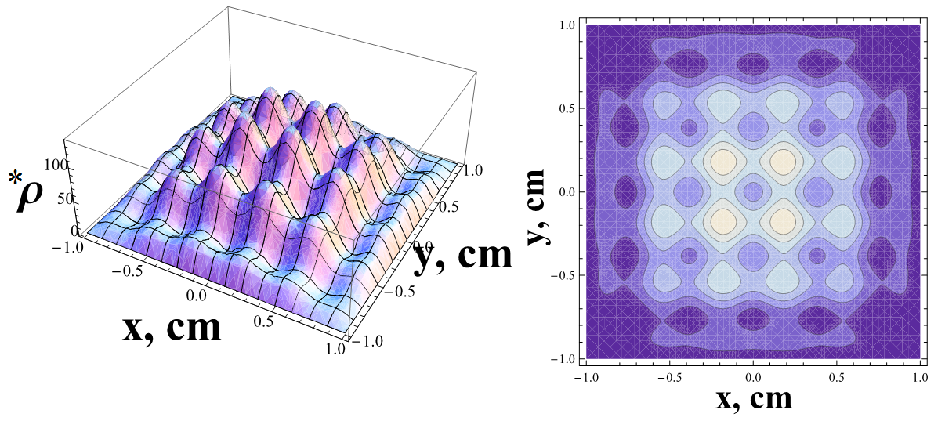
\includegraphics[width=8.5cm,height=4cm]{figures/002K.pdf}
\caption{The plot of the electron distribution function density. \\ $T=0.02\,K$, $\strut^*\!\rho=\rho/Q_{total}\cdot100\%$, no external field.}
\label{fig:1}
\end{figure}


Temperature growth makes possible to observe some smearing of electrons density function that conforms to our intuition (Fig.\ref{fig:2}).
Due to grounded boundaries, particles distribution function is always zero there, so we cannot expect uniform distribution function to be precisely a constant, but it tends to be as temperature and computation precision grow.
\begin{figure}[tbh]
\centering
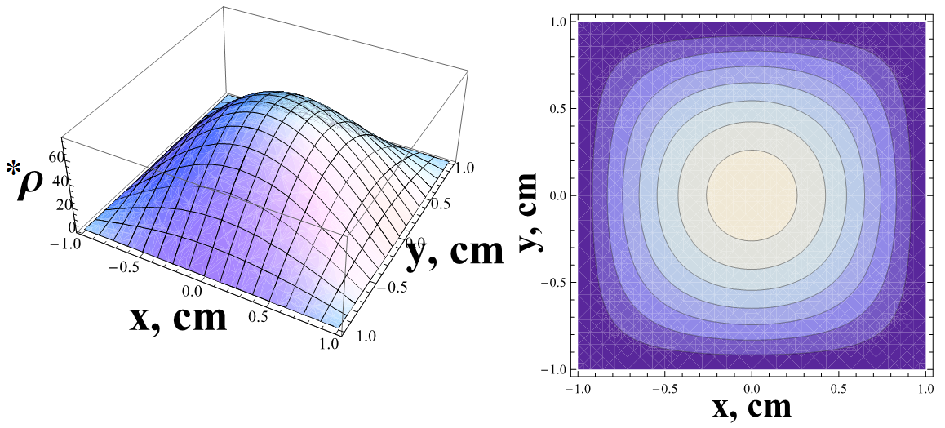
\includegraphics[width=8.5cm,height=4cm]{figures/04K.pdf}
\caption{The plot of the electron distribution function density.\\ $T=0.4\,K$, $\strut^*\!\rho=\rho/Q_{total}\cdot100\%$, no external field.}
\label{fig:2}
\end{figure}
 

It was mentioned that even without an external field there exist some inhomogeneities in distribution of electrons on the liquid helium surface.
Turning an external field on, can only deepen the difference between local maxima and minima of electron distribution function.
Computer simulation results again conform to intuition and show that some sharpening of density function can be observed (Fig.\ref{fig:3}). 
This means that electrons are collecting together due to some additional effective attraction. 
This is caused by helium film deformations.
External field presses electron into liquid helium, but due to some quantum effects they are pushed out of the helium. 
So electrons make helium film to "feel"\ external field and deform itself according to it.
Of course zones with higher particle concentration will be more deformed as zones with lower particles concentration.


But this is not the whole story.
Helium film deformations cause presence of some additional summand in this systems' free energy.
So deformations of the liquid helium film in the presence of external field will not only be some "sharpen"\ version of itself without an external field, rather system should find some form of the helium surface to minimize total free energy and it can qualitative differ from that without any field.  
(Fig.\ref{fig:3}) shows that local maxima and minima have shifted in addition to some sharpen.
When electrons density is big enough they can be pushed inside helium and form some kind of bubble full of electrons (bubblon).
Of course such behavior cannot be taken into account with so simple model, but some appropriate estimations can be done. 
\begin{figure}[tbh]
\centering
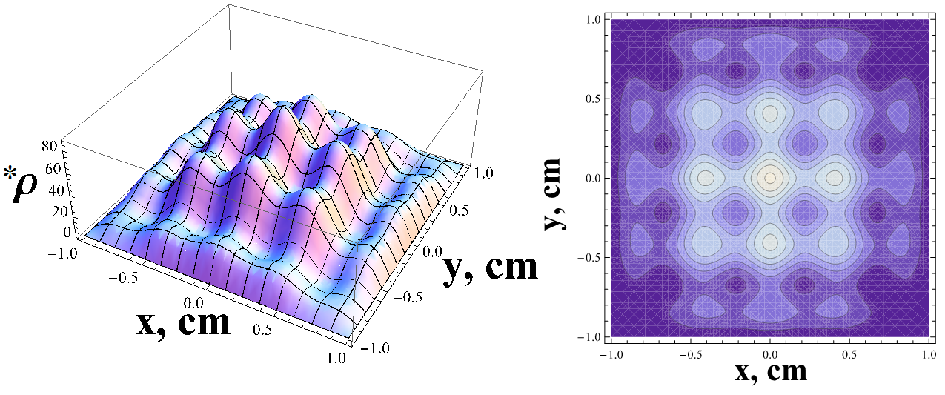
\includegraphics[width=8.5cm,height=4cm]{figures/cap10.pdf}
\caption{The plot of the electron distribution function density. \\ $T=0.02\,K$, $E=1.4 \cdot 10^5\, V/m$, $\strut^*\!\rho=\rho/Q_{total}\cdot100\%$.}
\label{fig:3}
\end{figure}


And last, but not the least. 
Suppose, that electrons concentration is low enough and external field is getting more and more stronger.
Numerical calculation show that if external field is strong enough this makes possible to collect almost all electrons in the center of the helium film  (Fig.\ref{fig:4}).
We can see that such distribution function is convex as for the case of high temperature without field.
The main difference between two distribution functions in his cases is that distribution function for the first case is very sharp and in the second case tends to become constant (Fig.\ref{fig:2}). 
\begin{figure}[tbh]
\centering
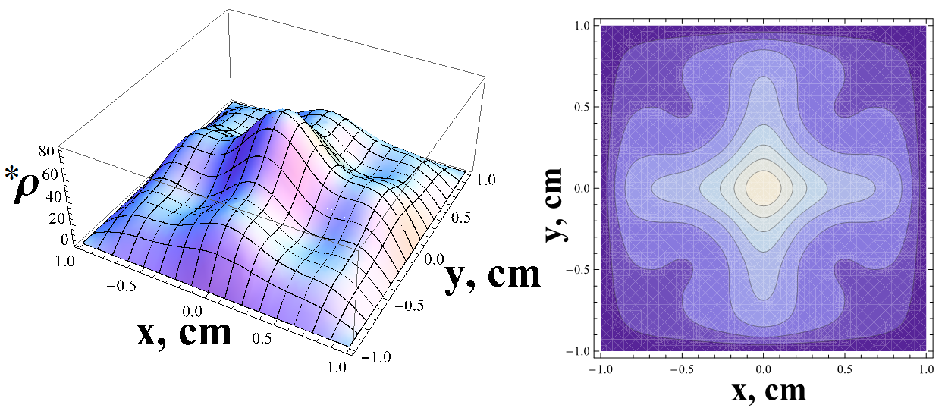
\includegraphics[width=8.5cm,height=4cm]{figures/cap20.pdf}
\caption{ The plot of the electron distribution function density.\\  $T=0.02\,K$, $E=2 \cdot 10^5\, V/m$, $\strut^*\!\rho=\rho/Q_{total}\cdot100\%$.}
\label{fig:4}
\end{figure}


This is significant qualitative change of electron distribution function (compare (Fig.\ref{fig:3}) and (Fig.\ref{fig:4})) and intensity of external electrical field when it is obtained can be treated as some critical value for this system to be stable.
This consists with possible analytical estimations ($E=2.03 \cdot 10^5\, V/m$ \cite{edelman}) 

\section{Conclusions}

There exists many possible methods for this system to be treated.
Most of them are based on quantum mechanics and quantum field theory and this causes their complexity.
But using electron potential on the liquid helium surface as some empirical data a simple quasiclassical model can be built.
This model can at least qualitatively predict some effects that can be observed on the liquid helium surface.
The other advantage is that it can be easily extended to other systems of interacting partricles, when we can neglect quantum correlations between particles and Bose-condensation, and allows easily build free energy functional in occupation numbers representation, so results are got directly in the view of density distribution.
Our model is simple enough to be resolved without using clusters or other powerful computer tools and with some additional simplifications can be even analyzed analytically. 


In addition to electrostatic forces between electrons and dielectric surface additional interaction through curve of the liquid helium surface was examined.
Though our approach is rather rough. 
First, we treated electrons as hard spheres of fixed radius.
Second, we assumed that many-particle interaction between electrons can be descripted with two-particle potential, many-particle interactions were neglected.
It can be right in approach of low-deformated surface, but it isn't good enough in the case of strong field.
Nevertheless this admission simplifies our calculations and leads to sufficient conclusions and obtained results are in agree with our intuition and existing experimental and theoretical works.


It was shown that ground state of the electron film isn't homogeneous.
Obtained results show, that presence and form of "metal walls"\ can significantly influence electron distribution function inducing some periodical structures in it.
If temperature grows we can see some smearing of this distribution function and it tends to be the uniform one when temperature is high enough.


Also importanse of electric field to the bubble formation was shown.
We saw, that taking surface deformation into account, which is negligible without external field, leads to essential changes in formed structures and to gathering of electrons to bigger structures, and the final point of such gathering is formation of a bubble.
If field is not strong enough, then only some sharpen of electron distribution function maxima can be observed.
This explains results, that were experimentally observed in~\cite{koutsoumpos}, especcialy division of the film into two liquids, that differently act in magnetic field.
Besides, this work doesn't detect the form of such division, only the fact of it.


We hope that modern experimental technique allows electrons distribution function on the liquid helium surface to be measured, and our results will be compared to experimental data.



\begin{thebibliography}{99}

\bibitem{edelman} V.S.Edel�man, Uspekhi Fizicheskikh Nauk {\bf 23}, 227 (1980).
\bibitem{ando_fowler_stern} T.Ando, A.Fowler, and F.Stern, Rev. Mod. Phys. {\bf 54}, 437 (1982).
\bibitem{alhassid} Y.Alhassid, Rev.Mod.Phys. {\bf 72}, 895 (2000).
\bibitem{luttinger} J.M.Luttinger, J.Math.Phys. {\bf 4}, 1154 (1963).
\bibitem{kroemer} H.Kroemer, Proc.IEEE {\bf 51}, 1782 (1963).
\bibitem{rupprecht_woodall_pettit} H.Rupprecht, J.M.Woodall, and G.D.Pettit, Appl.Phys.Lett. {\bf 11}, 81 (1967).
\bibitem{cole} M.W.Cole, Phys.Rev.B {\bf 2}, 4239 (1970).
\bibitem{cole_cohen} M.W.Cole and M.H.Cohen, Phys.Rev.Lett. {\bf 23}, 1238 (1969).
\bibitem{shikin} V.B.Shikin, Sov.Phys.JETP {\bf 31}, 939 (1970).
\bibitem{williams_crandall_willis} F.I.B.Williams, R.S.Crandall, and A.H.Willis, Phys.Rev.Lett. {\bf 26}, 7 (1971).
\bibitem{wigner} W.Wigner, Phys.Rev. {\bf 46}, 1002 (1934).
\bibitem{platzman_fukuyama} P.M.Platzman and H.Fukuyama, Phys.Rev. B {\bf 10}, 3150 (1974).
\bibitem{grimes_adams} C.C.Grimes {\it et al.}, Phys.Rev.Lett. {\bf 42}, 795 (1979).
\bibitem{klitzing_dorda_pepper} K.V.Klitzing, G.Dorda, and M.Pepper, Phys.Rev.Lett. {\bf 45}, 494 (1980).
\bibitem{tsui_stormer_gossard} D.C.Tsui, H.L.Stormer, and A.C.Gossard, Phys.Rev.Lett. {\bf 48}, 1559 (1982).
\bibitem{laughlin} R.B.Laughlin, Phys.Rev.Lett. {\bf 50}, 1395 (1983).
\bibitem{abrahams_etc} E.Abrahams, P.W.Anderson, D.C.Licciardello, and T.V.Ramakrishnan, Phys.Rev.Lett. {\bf 42}, 673 (1979).
\bibitem{tanatar_hakioglu} B.Tanatar and T.Hakioglu, Sol.St.Comm. {\bf 88}, 115 (1993).
\bibitem{zinn-justin} J.Zinn-Justin, Clarendon Press (1996).
\bibitem{datta} S.Datta, {\it Electronic transport in mesoscopic systems} (Cambridge University Press, 1995).
\bibitem{monarkha_kono} Yu.P.Monarkha and K.Kono, {\it Two-dimensional Coulomb liquids and solids} (Springer, 2004).
\bibitem{thouless} D.J.Thouless, Phys.Rep. {\bf 13}, 93 (1974).
\bibitem{GrainDynamics} B.I.Lev and A.G.Zagorodny, Phys.Lett. {\bf 373} (2009).
\bibitem{StronglyCollisional} B.I.Lev, V.B.Tymchyshyn, and A.G.Zagorodny, Cond.Matter Phys. {\bf 12} (2009).
\bibitem{myPublication} B.I.Lev, V.B.Tymchyshyn, and A.G.Zagorodny, Phys.Lett.A {\bf 375} (2011).
\bibitem{krasnoholovets_lev} V.Krasnoholovets and B.I.Lev, Cond.Matter Phys. {\bf 6}, 67 (2003).
\bibitem{platzman_dykman} P.M.Platzman and M.I.Dykman, Science {\bf 284}, 1967 (1999).
\bibitem{landau_lifshitz_8} L.D.Landau and E.M.Lifshitz, {\it Electrodynamics of continuous media} (Pergamon Press, 1984).
\bibitem{koutsoumpos} S.Koutsoumpos, {\it Surface State Electron Dynamics on Deformed Liquid Helium Films}, Ph.D. thesis, Konstanz (2010).
\bibitem{lambert} D.K.Lambert, {\it Electrons on the surface of liquid helium}, Ph.D. thesis, Lawrence Berkeley Laboratory (1979).
\bibitem{skachko} I.Skachko, {\it Phase diagram of a 2-dimensional electron system on the surface of liquid helium}, Ph.D. thesis, Rutgers, The State University of New Jersey (2006).
\bibitem{brown_grimes} T.R.Brown and C.C.Grimes, Phys.Rev.Lett. {\bf 29}, 1233 (1972).
\bibitem{rybalko_kovdrya_eselson} A.S.Rybalko, Yu.Z.Kovdrya, and B.N.Esel�son, JETP Lett. {\bf 22}, 280 (1976).
\bibitem{grimes_adams_1} C.C.Grimes and G.Adams, Phys.Rev.Lett. 1976(145).
\bibitem{kosterlitz_thouless} J.M.Kosterlitz and D.J.Thouless, J.Phys.C, 1181 (1973).
\bibitem{gorkov_chernikova} L.P.Gor'kov and D.M.Chernikova, JETP Lett. {\bf 18}, 119 (1973).
\bibitem{edwards_lennard} S.F.Edwards and A.Lennard, J.Math.Phys. {\bf 3}, 778 (1962).
\bibitem{samuel} S.Samuel, Phys.Rev. D {\bf 18}, 1916 (1978).
\bibitem{hubbard} J.Hubbard, Phys.Rev.Lett. {\bf 3}, 77 (1959).
\bibitem{lev_zhugayevich} B.I.Lev and A.Y.Zhugaevych, Phys.Rev. E 57, 6460 (1998).
\bibitem{gerson_etc} D.F.Gerson, J.E.Zaijc, M.D.Ouchi, and M. Ed., ACS symposium series, 66 (1979).
\bibitem{henry_prudich_vaidyanathan} J.D.Henry, M.E.Prudich, and K.R.Vaidyanathan, Sep.Purif.Methods {\bf 8}, 81 (1979).
\bibitem{nicolson} M.M.Nicolson, Proc. Cambridge Philos. Soc. {\bf 45}, 288 (1949).
\bibitem{kralchevsky_nagayama_1} P.A.Kralchevsky and K.Nagayama, Advances in Colloid and Interface Science {\bf 85}, 145 (2000).
\bibitem{chan_henry_white} D.Y.C.Chan, J.D.Henry, and L.R.White, J. Colloid Interface Sci. {\bf 79}, 410 (1981).
\bibitem{paunov_etc} V.N.Paunov, P.A.Kralchevsky, N.D.Denkov, and K.Nagayama, J. Colloid Interface Sci. {\bf 157}, 100 (1993).
\bibitem{kralchevsky_nagayama} P.A.Kralchevsky and K.Nagayama, Langmuir {\bf 10}, 23 (1994).
\bibitem{kralchevsky_etc} P.A.Kralchevsky, V.N.Paunov, N.D.Denkov, and K.Nagayama, J. Colloid Interface Sci. {\bf 167}, 47 (1994).


\end{thebibliography}


\end{document}

